\section{树的存储结构}

\begin{frame}\ft{\secname}
存储结构有两种方式,即顺序存储和链式存储。

\begin{itemize}
\item 顺序存储使用一段连续的存储单元依次存储各个数据元素。这对于线性表来说非常自然,但对树这样一对多的结构呢?
\item 树中某个结点的孩子可以有多个,这意味着,无论按何种顺序将树中所有结点存储到数组中,结点的存储位置都无法直接反映其逻辑关系。也就是说简单的顺序存储结构不能满足树的实现要求。
\end{itemize}
\end{frame}

\begin{frame}\ft{\secname}
我们可以充分利用顺序存储和链式存储结构的特点,来实现对树的存储结构的表示。
\end{frame}

\begin{frame}\ft{\secname}
\begin{itemize}
\item 双亲表示法
\item 孩子表示法
\item 孩子兄弟表示法
\end{itemize}
\end{frame}
 
\begin{frame}\ft{双亲表示法}
假设用一组连续空间来存储树的结点,同时在每个结点中附设一个指示器,以指示其双亲结点在数组中的位置。也就是说,每个结点除了知道自己是谁以外,还需知道其双亲在哪儿。 \vspace{0.1in}

\begin{figure}
\begin{tikzpicture}
  \def\x{1.5}\def\y{0.8}
  \draw[very thick](0,0)rectangle(2*\x,\y) (\x,0)--(\x,\y);
  \node at (0.5*\x,0.5*\y) [] { data};
  \node at (1.5*\x,0.5*\y) [] { parent};

  \tikzstyle{every node}=[]
  \tikzstyle{information text}=[rounded corners,inner sep=1ex]
  \draw
  node at (\x,0.*\y) [below=0.2cm,text width=10cm,style=information text]
  {
    \begin{table}
      \centering
      \begin{tabular}{l|l|l} \hline
         data & 数据域 & 存储结点的数据信息  \\[0.1in]
         parent & 指针域 & 存储该结点的双亲在数组中的下标  \\\hline
      \end{tabular}      
    \end{table}
  };
\end{tikzpicture}
        
\caption{双亲表示法的结点结构}

\end{figure}
\end{frame}

\begin{frame}\ft{双亲表示法}
\lstinputlisting[
language=C,
]{Chapters/Ch04/Code/Storage/parent.h}
\end{frame}
%
\begin{frame}\ft{双亲表示法}
由于根结点没有双亲,约定其指针域为$-1$,也就是说,所有结点都存有其双亲的位置。
\end{frame}

\begin{frame}\ft{双亲表示法}
\begin{small}
\begin{minipage}[t]{0.45\textwidth}
\begin{figure}
\centering
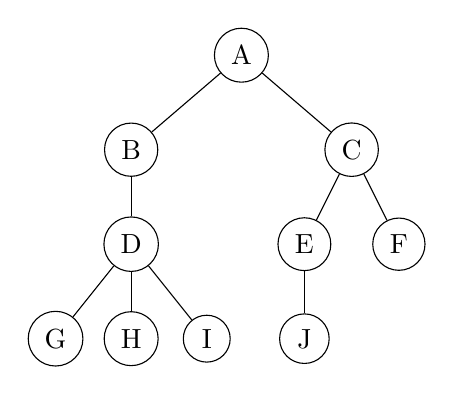
\begin{tikzpicture}[scale=0.8]
  
  %% \tikzstyle{every node}=[ball color=red!70,circle,text=white]
  
  \node [circle,draw] at (0,0) {A}[sibling distance=3.5cm] 
  child { node[circle,draw]{B}
    child {node[circle,draw]{D}[sibling distance=1.2cm]
      child {node[circle,draw]{G}}
      child {node[circle,draw]{H}}
      child {node[circle,draw]{I}}
    }
  }
  child { node[circle,draw]{C}[sibling distance=1.5cm]          
    child {node[circle,draw]{E}
      child {node[circle,draw]{J}} 
    }
    child {node[circle,draw]{F}} 
  };
\end{tikzpicture}
        
\end{figure}
\end{minipage}
\begin{minipage}[t]{0.45\textwidth}
\begin{table}
\begin{tabular}{c|c|c}\hline
 index & data & parent\\\hline
0&A&-1\\
1&B&0\\
2&C&0\\
3&D&1\\
4&E&2\\
5&F&2\\
6&G&3\\
7&H&3\\
8&I&3\\
9&J&4\\\hline
\end{tabular}
\end{table}
\end{minipage}
\end{small}
\end{frame}

\begin{frame}\ft{双亲表示法}
这样的存储结构,根据结点的parent指针可以很容易找到其双亲结点,时间复杂度为$O(1)$。当parent为$-1$时,表示找到了根结点。 \vspace{0.2in}

但是,若想知道结点的孩子是什么,则必须遍历整个结构。
\end{frame}
%
%
\begin{frame}\ft{双亲表示法+长子域}
\textcolor{acolor3}{改进:}

增加一个最左边孩子的域,不妨称之为\textcolor{acolor3}{长子域},这样就可以很容易找到结点的孩子。若该结点没有孩子,其长子域就设为$-1$。
\end{frame}
%
%
\begin{frame}\ft{双亲表示法+长子域}
\begin{small}
\begin{minipage}[t]{0.45\textwidth}
\begin{figure}
\centering
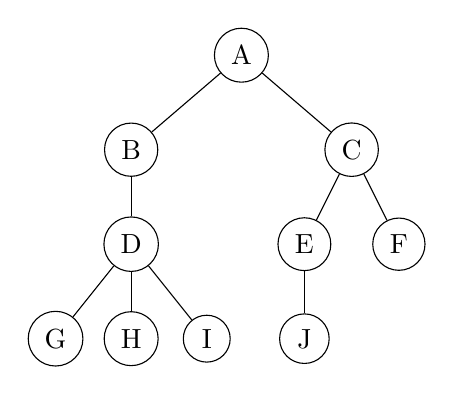
\begin{tikzpicture}[scale=0.8]
  
  %% \tikzstyle{every node}=[ball color=red!70,circle,text=white]
  
  \node [circle,draw] at (0,0) {A}[sibling distance=3.5cm] 
  child { node[circle,draw]{B}
    child {node[circle,draw]{D}[sibling distance=1.2cm]
      child {node[circle,draw]{G}}
      child {node[circle,draw]{H}}
      child {node[circle,draw]{I}}
    }
  }
  child { node[circle,draw]{C}[sibling distance=1.5cm]          
    child {node[circle,draw]{E}
      child {node[circle,draw]{J}} 
    }
    child {node[circle,draw]{F}} 
  };
\end{tikzpicture}
        
\end{figure}
\end{minipage}
\begin{minipage}[t]{0.45\textwidth}
\begin{table}
\begin{tabular}{c|c|c|c}\hline
index & data & parent & firstchild\\\hline
0&A&-1&1\\
1&B&0 &3\\
2&C&0 &4\\
3&D&1 &6\\
4&E&2 &9\\
5&F&2 &-1\\
6&G&3 &-1\\
7&H&3 &-1\\
8&I&3 &-1\\
9&J&4 &-1\\\hline
\end{tabular}
\end{table}
\end{minipage}
\end{small}
\end{frame}
%
%
\begin{frame}\ft{双亲表示法+右兄弟域}
如若关注各兄弟之间的关系,可增加一个右兄弟域来体现兄弟关系,亦即,某个结点若存在右兄弟,则记录下其右兄弟的下标;若不存在,则赋值为$-1$。
\end{frame}

\begin{frame}\ft{双亲表示法+右兄弟域}
\begin{small}
\begin{minipage}[t]{0.45\textwidth}
\begin{figure}
\centering
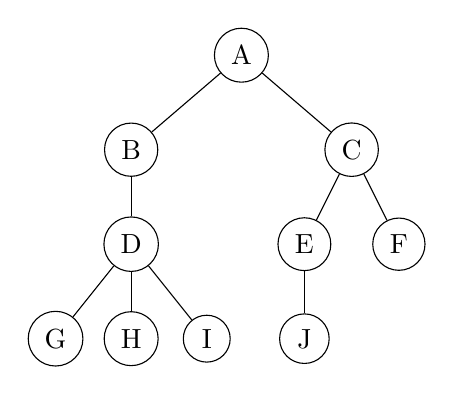
\begin{tikzpicture}[scale=0.8]
  
  %% \tikzstyle{every node}=[ball color=red!70,circle,text=white]
  
  \node [circle,draw] at (0,0) {A}[sibling distance=3.5cm] 
  child { node[circle,draw]{B}
    child {node[circle,draw]{D}[sibling distance=1.2cm]
      child {node[circle,draw]{G}}
      child {node[circle,draw]{H}}
      child {node[circle,draw]{I}}
    }
  }
  child { node[circle,draw]{C}[sibling distance=1.5cm]          
    child {node[circle,draw]{E}
      child {node[circle,draw]{J}} 
    }
    child {node[circle,draw]{F}} 
  };
\end{tikzpicture}
        
\end{figure}
\end{minipage}
\begin{minipage}[t]{0.45\textwidth}
\begin{table}
\begin{tabular}{c|c|c|c}\hline
index &data &parent &rightsib\\\hline
0&A&-1&-1\\
1&B&0 &2\\
2&C&0 &-1\\
3&D&1 &-1\\
4&E&2 &5\\
5&F&2 &-1\\
6&G&3 &7\\
7&H&3 &8\\
8&I&3 &-1\\
9&J&4 &-1\\\hline
\end{tabular}
\end{table}
\end{minipage}
\end{small}
\end{frame}
%
\begin{frame}\ft{双亲表示法+右兄弟域}
若结点的孩子很多,超过了2个。但我们又关注结点的双亲、结点的孩子以及结点的兄弟,并且对时间遍历要求还比较高,那我们可以把此结构扩展为有双亲域、长子域以及右兄弟域。
\end{frame}
%
\begin{frame}\ft{\secname}
存储结构的设计是一个非常灵活的过程。一个存储结构设计得是否合理,取决于基于该存储结构的运算是否适合、是否方便,时间复杂度好不好等。
但也不是越多越好。
\end{frame}
%
%
%\subsection{孩子表示法}
%
\begin{frame}\ft{孩子表示法}
由于树中每个结点可能有多棵子树,可以考虑用多重链表,即\textcolor{acolor4}{每个结点有多个指针域,其中每个指针指向一颗子树的根结点,该方法称为多重链表表示法。} \vspace{0.2in}

不过,树的每个结点的度,即其孩子是不同的,可以考虑如下两种方案。
\end{frame}
%
\begin{frame}\ft{孩子表示法}
\textcolor{acolor3}{方案一:}
指针域的个数等于树的度。
\begin{figure}
\centering
\begin{tikzpicture}
  \def\x{1.5}\def\y{0.8}
  \draw[very thick](0,0)rectangle(6*\x,\y);
  \foreach \i in {1,2,...,5}
  \draw[very thick](\i*\x,0)--(\i*\x,\y);
  \node at (0.5*\x,0.5*\y) [] {\tt data};
  \node at (1.5*\x,0.5*\y) [] {\tt child1};
  \node at (2.5*\x,0.5*\y) [] {\tt child2};
  \node at (3.5*\x,0.5*\y) [] {\tt child3};
  \node at (4.5*\x,0.5*\y) [] {$\cd$};
  \node at (5.5*\x,0.5*\y) [] {\tt childd};
  \tikzstyle{every node}=[]
  \tikzstyle{information text}=[rounded corners,inner sep=1ex]
  \draw
  node at (3*\x,0.*\y) [below=0.2cm,text width=10cm,style=information text]
  {
    \begin{table}
      \centering
      \begin{tabular}{l|l|l} \hline
         {\tt data} & 数据域 & 存储结点的数据信息  \\[0.1in]
         {\tt child1-childd} & 指针域 & 指向该结点的各个孩子的结点  \\\hline
      \end{tabular}      
    \end{table}
  };
\end{tikzpicture}
        
\end{figure}
\end{frame}
%

\begin{frame}\ft{孩子表示法}
\begin{small}
\begin{figure}
\centering
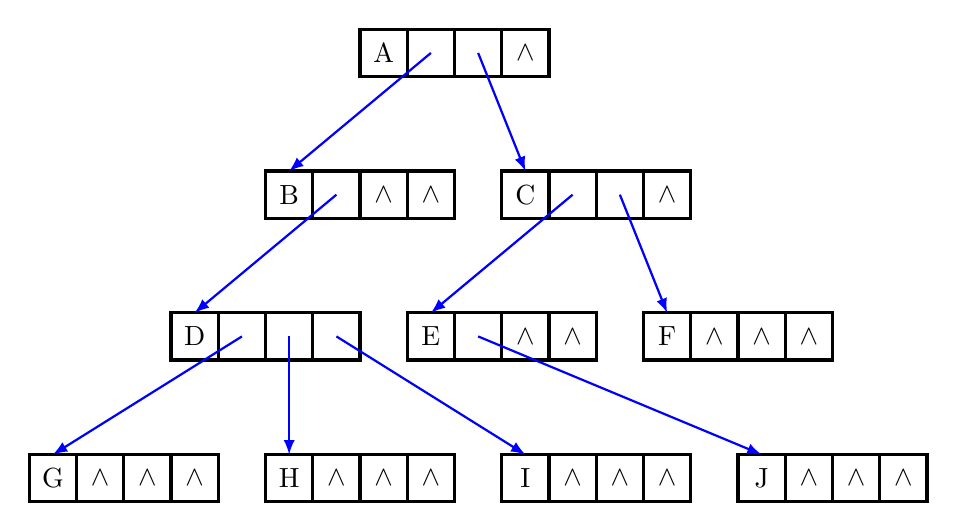
\begin{tikzpicture}[scale=1]
  \def\x{0.6} \def\y{0.6}
  %% \draw[dashed,step=\x] (0*\x,0*\y) grid (20*\x,12*\y);


  \foreach \i in {0,5,10,15}{
    \def\j{0}
    \draw[very thick](\i*\x,\j*\y)rectangle(\i*\x+4*\x,\j*\y+\y)
    (\i*\x+\x,\j*\y)--(\i*\x+\x,\j*\y+\y)
    (\i*\x+2*\x,\j*\y)--(\i*\x+2*\x,\j*\y+\y)
    (\i*\x+3*\x,\j*\y)--(\i*\x+3*\x,\j*\y+\y);
    \node at(\i*\x+1.5*\x,\j*\y+0.5*\y)[]{$\land$};
    \node at(\i*\x+2.5*\x,\j*\y+0.5*\y)[]{$\land$};
    \node at(\i*\x+3.5*\x,\j*\y+0.5*\y)[]{$\land$};
    
  }
  \def\i{0}\def\j{0}
  \node at(\i*\x+0.5*\x,\j*\y+0.5*\y)[]{G};

  \def\i{5}\def\j{0}
  \node at(\i*\x+0.5*\x,\j*\y+0.5*\y)[]{H};
  
  \def\i{10}\def\j{0}
  \node at(\i*\x+0.5*\x,\j*\y+0.5*\y)[]{I};
  
  \def\i{15}\def\j{0}
  \node at(\i*\x+0.5*\x,\j*\y+0.5*\y)[]{J};

  
  \foreach \i in {3,8,13}{
    \def\j{3}
    \draw[very thick](\i*\x,\j*\y)rectangle(\i*\x+4*\x,\j*\y+\y)
    (\i*\x+\x,\j*\y)--(\i*\x+\x,\j*\y+\y)
    (\i*\x+2*\x,\j*\y)--(\i*\x+2*\x,\j*\y+\y)
    (\i*\x+3*\x,\j*\y)--(\i*\x+3*\x,\j*\y+\y);
  }


  \def\i{3}\def\j{3}
  \node at(\i*\x+0.5*\x,\j*\y+0.5*\y)[]{D};
  \draw[blue,thick,->,>=latex] (\i*\x+1.5*\x,\j*\y+0.5*\y)--(0*\x+0.5*\x,\j*\y-2*\y);
  \draw[blue,thick,->,>=latex] (\i*\x+2.5*\x,\j*\y+0.5*\y)--(5*\x+0.5*\x,\j*\y-2*\y);
  \draw[blue,thick,->,>=latex] (\i*\x+3.5*\x,\j*\y+0.5*\y)--(10*\x+0.5*\x,\j*\y-2*\y);
  
  \def\i{8}\def\j{3}
  \node at(\i*\x+0.5*\x,\j*\y+0.5*\y)[]{E};
  \node at(\i*\x+2.5*\x,\j*\y+0.5*\y)[]{$\land$};
  \node at(\i*\x+3.5*\x,\j*\y+0.5*\y)[]{$\land$};
  \draw[blue,thick,->,>=latex] (\i*\x+1.5*\x,\j*\y+0.5*\y)--(15*\x+0.5*\x,\j*\y-2*\y);
  
  \def\i{13}\def\j{3}
  \node at(\i*\x+0.5*\x,\j*\y+0.5*\y)[]{F};
  \node at(\i*\x+1.5*\x,\j*\y+0.5*\y)[]{$\land$};
  \node at(\i*\x+2.5*\x,\j*\y+0.5*\y)[]{$\land$};
  \node at(\i*\x+3.5*\x,\j*\y+0.5*\y)[]{$\land$};

  \foreach \i in {5,10}{
    \def\j{6}
    \draw[very thick](\i*\x,\j*\y)rectangle(\i*\x+4*\x,\j*\y+\y)
    (\i*\x+\x,\j*\y)--(\i*\x+\x,\j*\y+\y)
    (\i*\x+2*\x,\j*\y)--(\i*\x+2*\x,\j*\y+\y)
    (\i*\x+3*\x,\j*\y)--(\i*\x+3*\x,\j*\y+\y);
  }

  \def\i{5}\def\j{6}
  \node at(\i*\x+0.5*\x,\j*\y+0.5*\y)[]{B};
  \draw[blue,thick,->,>=latex] (\i*\x+1.5*\x,\j*\y+0.5*\y)--(3*\x+0.5*\x,\j*\y-2*\y);
  \node at(\i*\x+2.5*\x,\j*\y+0.5*\y)[]{$\land$};
  \node at(\i*\x+3.5*\x,\j*\y+0.5*\y)[]{$\land$};
  
  \def\i{10}\def\j{6}
  \node at(\i*\x+0.5*\x,\j*\y+0.5*\y)[]{C};
  \draw[blue,thick,->,>=latex] (\i*\x+1.5*\x,\j*\y+0.5*\y)--(8*\x+0.5*\x,\j*\y-2*\y);
  \draw[blue,thick,->,>=latex] (\i*\x+2.5*\x,\j*\y+0.5*\y)--(13*\x+0.5*\x,\j*\y-2*\y);
  \node at(\i*\x+3.5*\x,\j*\y+0.5*\y)[]{$\land$};


  \foreach \i in {7}{
    \def\j{9}
    \draw[very thick](\i*\x,\j*\y)rectangle(\i*\x+4*\x,\j*\y+\y)
    (\i*\x+\x,\j*\y)--(\i*\x+\x,\j*\y+\y)
    (\i*\x+2*\x,\j*\y)--(\i*\x+2*\x,\j*\y+\y)
    (\i*\x+3*\x,\j*\y)--(\i*\x+3*\x,\j*\y+\y);
  }
  \def\i{7}\def\j{9}
  \node at(\i*\x+0.5*\x,\j*\y+0.5*\y)[]{A};
  \node at(\i*\x+3.5*\x,\j*\y+0.5*\y)[]{$\land$};
  \draw[blue,thick,->,>=latex] (\i*\x+1.5*\x,\j*\y+0.5*\y)--(5*\x+0.5*\x,\j*\y-2*\y);
  \draw[blue,thick,->,>=latex] (\i*\x+2.5*\x,\j*\y+0.5*\y)--(10*\x+0.5*\x,\j*\y-2*\y);
  
\end{tikzpicture}

\caption{多重链表表示法1:固定指针域}
\end{figure}
\end{small}
\end{frame}
%
%
\begin{frame}\ft{孩子表示法}
当各结点的度相差很大时,该方法显然是浪费空间的。不过,当各结点的度相差很小时,开辟的空间得以充分利用,此存储结构的缺点反而成了优点。\vspace{0.2in}

\pause 
\begin{wenti}
如果很多指针域为空,为什么不能按需分配呢?
\end{wenti}
\end{frame}
%
\begin{frame}\ft{孩子表示法}
\textcolor{acolor3}{方案二:}
每个结点的指针域的个数等于该结点的度,专门取一个位置来存储结点指针域的个数。
\begin{figure}
\centering
\begin{tikzpicture}
  \def\x{1.5}\def\y{0.8}
  \draw[very thick](0,0)rectangle(7*\x,\y);
  \foreach \i in {1,2,...,6}
  \draw[very thick](\i*\x,0)--(\i*\x,\y);
  \node at (0.5*\x,0.5*\y) [] {\tt data};
  \node at (1.5*\x,0.5*\y) [] {\tt degree};
  \node at (2.5*\x,0.5*\y) [] {\tt child1};
  \node at (3.5*\x,0.5*\y) [] {\tt child2};
  \node at (4.5*\x,0.5*\y) [] {\tt child3};
  \node at (5.5*\x,0.5*\y) [] {$\cd$};
  \node at (6.5*\x,0.5*\y) [] {\tt childd};
  \tikzstyle{every node}=[]
  \tikzstyle{information text}=[rounded corners,inner sep=1ex]
  \draw
  node at (3.5*\x,0.*\y) [below=0.2cm,text width=10cm,style=information text]
  {
    \begin{table}
      \centering
      \begin{tabular}{l|l|l} \hline
         {\tt data} & 数据域 & 存储结点的数据信息  \\[0.1in]
         {\tt degree} & 度域 & 存储该结点的孩子的个数\\[0.1in]
         {\tt child1-childd} & 指针域 & 指向该结点的各个孩子的结点  \\\hline
      \end{tabular}
      
    \end{table}
  };
\end{tikzpicture}
        
\end{figure}

\end{frame}
%
\begin{frame}\ft{孩子表示法}
\begin{figure}
\centering
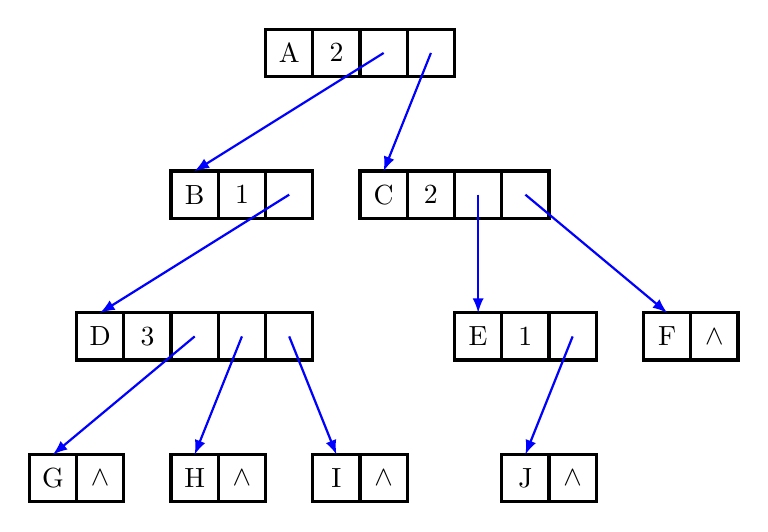
\begin{tikzpicture}[scale=1]
  \def\x{0.6} \def\y{0.6}
  %% \draw[dashed,step=\x] (0*\x,0*\y) grid (16*\x,12*\y);

  %%%%%%%%%Level 4%%%%%%%%%
  \foreach \i in {0,3,6,10}{
    \def\j{0}
    \draw[very thick](\i*\x,\j*\y)rectangle(\i*\x+2*\x,\j*\y+\y)
    (\i*\x+\x,\j*\y)--(\i*\x+\x,\j*\y+\y);
    \node at(\i*\x+1.5*\x,\j*\y+0.5*\y)[]{$\land$};    
  }
  \def\i{0}\def\j{0}
  \node at(\i*\x+0.5*\x,\j*\y+0.5*\y)[]{G};

  \def\i{3}\def\j{0}
  \node at(\i*\x+0.5*\x,\j*\y+0.5*\y)[]{H};
  
  \def\i{6}\def\j{0}
  \node at(\i*\x+0.5*\x,\j*\y+0.5*\y)[]{I};
  
  \def\i{10}\def\j{0}
  \node at(\i*\x+0.5*\x,\j*\y+0.5*\y)[]{J};

  %%%%%%%%%Level 3%%%%%%%%% 
  \def\i{1}\def\j{3}
  \draw[very thick](\i*\x,\j*\y)rectangle(\i*\x+5*\x,\j*\y+\y)
  (\i*\x+\x,\j*\y)--(\i*\x+\x,\j*\y+\y)
  (\i*\x+2*\x,\j*\y)--(\i*\x+2*\x,\j*\y+\y)
  (\i*\x+3*\x,\j*\y)--(\i*\x+3*\x,\j*\y+\y)
  (\i*\x+4*\x,\j*\y)--(\i*\x+4*\x,\j*\y+\y);
  \node at(\i*\x+0.5*\x,\j*\y+0.5*\y)[]{D};
  \node at(\i*\x+1.5*\x,\j*\y+0.5*\y)[]{3};
  \draw[blue,thick,->,>=latex] (\i*\x+2.5*\x,\j*\y+0.5*\y)--(0*\x+0.5*\x,\j*\y-2*\y);
  \draw[blue,thick,->,>=latex] (\i*\x+3.5*\x,\j*\y+0.5*\y)--(3*\x+0.5*\x,\j*\y-2*\y);
  \draw[blue,thick,->,>=latex] (\i*\x+4.5*\x,\j*\y+0.5*\y)--(6*\x+0.5*\x,\j*\y-2*\y);

  \def\i{9}\def\j{3}
  \draw[very thick](\i*\x,\j*\y)rectangle(\i*\x+3*\x,\j*\y+\y)
  (\i*\x+\x,\j*\y)--(\i*\x+\x,\j*\y+\y)
  (\i*\x+2*\x,\j*\y)--(\i*\x+2*\x,\j*\y+\y);
  \node at(\i*\x+0.5*\x,\j*\y+0.5*\y)[]{E};
  \node at(\i*\x+1.5*\x,\j*\y+0.5*\y)[]{1};
  \draw[blue,thick,->,>=latex] (\i*\x+2.5*\x,\j*\y+0.5*\y)--(10*\x+0.5*\x,\j*\y-2*\y);
  
  \def\i{13}\def\j{3}
  \draw[very thick](\i*\x,\j*\y)rectangle(\i*\x+2*\x,\j*\y+\y)
  (\i*\x+\x,\j*\y)--(\i*\x+\x,\j*\y+\y);
  \node at(\i*\x+0.5*\x,\j*\y+0.5*\y)[]{F};
  \node at(\i*\x+1.5*\x,\j*\y+0.5*\y)[]{$\land$};

  %%%%%%%%%Level 2%%%%%%%%%
  \def\i{3}\def\j{6}
  \draw[very thick](\i*\x,\j*\y)rectangle(\i*\x+3*\x,\j*\y+\y)
  (\i*\x+\x,\j*\y)--(\i*\x+\x,\j*\y+\y)
  (\i*\x+2*\x,\j*\y)--(\i*\x+2*\x,\j*\y+\y);
  \node at(\i*\x+0.5*\x,\j*\y+0.5*\y)[]{B};
  \node at(\i*\x+1.5*\x,\j*\y+0.5*\y)[]{1};
  \draw[blue,thick,->,>=latex] (\i*\x+2.5*\x,\j*\y+0.5*\y)--(1*\x+0.5*\x,\j*\y-2*\y);
  
  \def\i{7}\def\j{6}
  \draw[very thick](\i*\x,\j*\y)rectangle(\i*\x+4*\x,\j*\y+\y)
  (\i*\x+\x,\j*\y)--(\i*\x+\x,\j*\y+\y)
  (\i*\x+2*\x,\j*\y)--(\i*\x+2*\x,\j*\y+\y)
  (\i*\x+3*\x,\j*\y)--(\i*\x+3*\x,\j*\y+\y);
  \node at(\i*\x+0.5*\x,\j*\y+0.5*\y)[]{C};
  \node at(\i*\x+1.5*\x,\j*\y+0.5*\y)[]{2};
  \draw[blue,thick,->,>=latex] (\i*\x+2.5*\x,\j*\y+0.5*\y)--(9*\x+0.5*\x,\j*\y-2*\y);
  \draw[blue,thick,->,>=latex] (\i*\x+3.5*\x,\j*\y+0.5*\y)--(13*\x+0.5*\x,\j*\y-2*\y);

  %%%%%%%%%Level 1%%%%%%%%%
  \def\i{5}\def\j{9}
  \draw[very thick](\i*\x,\j*\y)rectangle(\i*\x+4*\x,\j*\y+\y)
  (\i*\x+\x,\j*\y)--(\i*\x+\x,\j*\y+\y)
  (\i*\x+2*\x,\j*\y)--(\i*\x+2*\x,\j*\y+\y)
  (\i*\x+3*\x,\j*\y)--(\i*\x+3*\x,\j*\y+\y);
  \node at(\i*\x+0.5*\x,\j*\y+0.5*\y)[]{A};
  \node at(\i*\x+1.5*\x,\j*\y+0.5*\y)[]{2};
  \draw[blue,thick,->,>=latex] (\i*\x+2.5*\x,\j*\y+0.5*\y)--(3*\x+0.5*\x,\j*\y-2*\y);
  \draw[blue,thick,->,>=latex] (\i*\x+3.5*\x,\j*\y+0.5*\y)--(7*\x+0.5*\x,\j*\y-2*\y);
  
\end{tikzpicture}

\caption{多重链表表示法2:按需分配指针域}
\end{figure}
\end{frame}
%
\begin{frame}\ft{孩子表示法}
该方法克服了空间浪费的缺点,但由于各个结点的链表结构不同,需要维护结点度的值,在运算上会带来时间上的损耗。\vspace{0.2in}

\pause 
\begin{wenti}
能否有更好的办法,既可以减少空指针的浪费又能使结点结构相同?
\end{wenti}\vspace{0.2in}

\pause
为了遍历整棵树,可以把结点放在一个顺序存储结构的数组中,但每个结点的孩子有多少不确定,可以再对每个结点的孩子建立一个单链表来体现它们的关系。
\end{frame}
%
%
%
\begin{frame}\ft{孩子表示法}

把每个结点的孩子排列起来,以单链表做存储结构,$n$个结点有$n$个孩子链表,如果是叶子结点则此单链表为空。

而$n$个结点组成一个线性表,采用顺序存储结构,存放在一个一维数组中。
\end{frame}

\begin{frame}\ft{孩子表示法}
为此,设计两种结点结构: \vspace{0.1in}

1、孩子链表的孩子结点:\vspace{0.1in}

\begin{figure}
\centering
\begin{tikzpicture}
  \def\x{1.5}\def\y{0.8}
  \draw[very thick](0,0)rectangle(2*\x,\y) (\x,0)--(\x,\y);
  \node at (0.5*\x,0.5*\y) [] {\tt child};
  \node at (1.5*\x,0.5*\y) [] {\tt next};

  \tikzstyle{every node}=[]
  \tikzstyle{information text}=[rounded corners,inner sep=1ex]

  \draw
  node at (1*\x,0*\y) [below,text width=10cm,style=information text]
  {
    \begin{table}
      \centering
      \begin{tabular}{l|l|l} \hline
         {\tt child} & 数据域 & 存储某个结点在表头数组中的下标 \\[0.1in]
         {\tt next} & 指针域 & 存储指向某结点的下一个孩子的指针 \\\hline
      \end{tabular}
      
    \end{table}
  };

\end{tikzpicture}
        
\end{figure}
\end{frame}

\begin{frame}\ft{\subsecname}
2、表头数组的表头结点:\vspace{0.1in}

\begin{figure}
\centering
\begin{tikzpicture}
  \def\x{3}\def\y{0.8}
  \draw[very thick](0,0)rectangle(2*\x,\y) (\x,0)--(\x,\y);
  \node at (0.5*\x,0.5*\y) [] {\tt data};
  \node at (1.5*\x,0.5*\y) [] {\tt firstchild};

  \tikzstyle{every node}=[]
  \tikzstyle{information text}=[rounded corners,inner sep=1ex]
  \draw
  node at (0.5*\x,0*\y) [below=0.2cm,text width=10cm,style=information text]
  {
    \begin{table}
      \centering
      \begin{tabular}{l|l|l} \hline
         {\tt data} & 数据域 & 存储结点的数据信息  \\[0.1in]
         {\tt firstchild} & 头指针域 & 存储该结点的孩子链表的头指针 \\\hline
      \end{tabular}
      
    \end{table}
  };
\end{tikzpicture}
        
\end{figure}
\end{frame}
%
%
%
%

\begin{frame}\ft{孩子表示法}
\begin{figure}
\centering
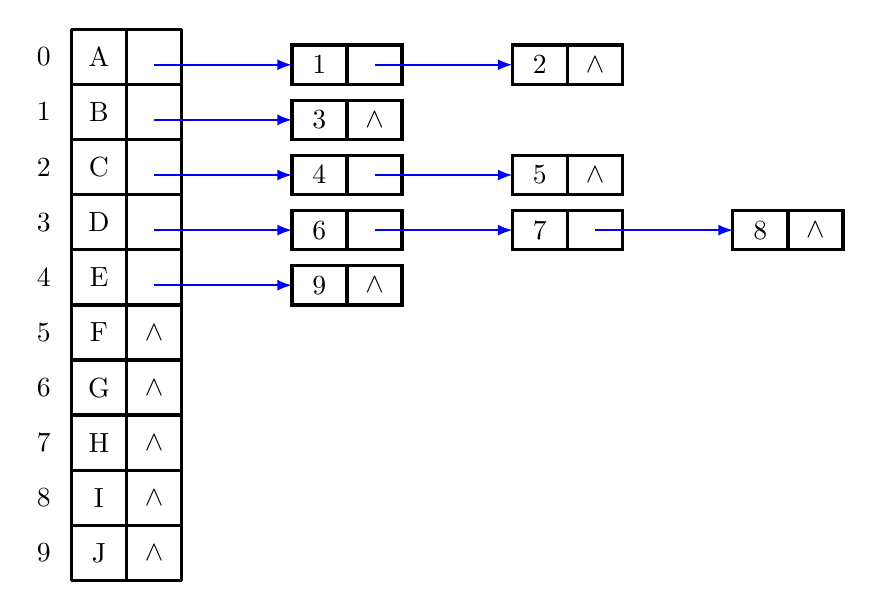
\begin{tikzpicture}[scale=1]
  \def\x{0.7} \def\y{0.7} \def\yy{0.5}
  %% \draw[dashed,step=\x] (0*\x,0*\y) grid (16*\x,10*\y);
  
  \draw[very thick,step=\x] (1*\x,0*\y) grid (3*\x,10*\y);
  \foreach \i in {0,1,2,...,9}
  \node at(0.5*\x,9.5*\y-\i*\y)[]{\i};

  \foreach \j in {9,8,7,6,5}
  \draw[very thick,step=\x] (5*\x,\j*\y) rectangle (7*\x,\j*\y+\yy)
  (6*\x,\j*\y)--(6*\x,\j*\y+\yy);

  \foreach \j in {9,7,6}
  \draw[very thick,step=\x] (9*\x,\j*\y) rectangle (11*\x,\j*\y+\yy)
  (10*\x,\j*\y)--(10*\x,\j*\y+\yy);

  \foreach \j in {6}
  \draw[very thick,step=\x] (13*\x,\j*\y) rectangle (15*\x,\j*\y+\yy)
  (14*\x,\j*\y)--(14*\x,\j*\y+\yy);
  
  \node at(1.5*\x,0.5*\y)[]{J}; 
  \node at(1.5*\x,1.5*\y)[]{I}; 
  \node at(1.5*\x,2.5*\y)[]{H}; 
  \node at(1.5*\x,3.5*\y)[]{G}; 
  \node at(1.5*\x,4.5*\y)[]{F}; 
  \node at(1.5*\x,5.5*\y)[]{E}; \node at(5.5*\x,5*\y+0.5*\yy)[]{9};  
  \node at(1.5*\x,6.5*\y)[]{D}; \node at(5.5*\x,6*\y+0.5*\yy)[]{6}; \node at(9.5*\x,6*\y+0.5*\yy)[]{7}; \node at(13.5*\x,6*\y+0.5*\yy)[]{8}; 
  \node at(1.5*\x,7.5*\y)[]{C}; \node at(5.5*\x,7*\y+0.5*\yy)[]{4}; \node at(9.5*\x,7*\y+0.5*\yy)[]{5}; 
  \node at(1.5*\x,8.5*\y)[]{B}; \node at(5.5*\x,8*\y+0.5*\yy)[]{3}; 
  \node at(1.5*\x,9.5*\y)[]{A}; \node at(5.5*\x,9*\y+0.5*\yy)[]{1}; \node at(9.5*\x,9*\y+0.5*\yy)[]{2}; 

  \def\i{1}
  \foreach \j in {0,1,2,3,4}
  \node at(\i*\x+1.5*\x,\j*\y+0.5*\y)[]{$\land$};
  \foreach \j in {5,6,7,8,9}
  \draw[blue,thick,->,>=latex](\i*\x+1.5*\x,\j*\y+0.5*\yy)--(\i*\x+4*\x,\j*\y+0.5*\yy);

  \def\i{5}
  \foreach \j in {5,8}
  \node at(\i*\x+1.5*\x,\j*\y+0.5*\yy)[]{$\land$};
  \foreach \j in {6,7,9}
  \draw[blue,thick,->,>=latex](\i*\x+1.5*\x,\j*\y+0.5*\yy)--(\i*\x+4*\x,\j*\y+0.5*\yy);

  \def\i{9}
  \foreach \j in {9,7}
  \node at(\i*\x+1.5*\x,\j*\y+0.5*\yy)[]{$\land$};
  \foreach \j in {6}
  \draw[blue,thick,->,>=latex](\i*\x+1.5*\x,\j*\y+0.5*\yy)--(\i*\x+4*\x,\j*\y+0.5*\yy);

  \def\i{13}
  \foreach \j in {6}
  \node at(\i*\x+1.5*\x,\j*\y+0.5*\yy)[]{$\land$};

\end{tikzpicture}

%\caption{孩子表示法}
\end{figure}
\end{frame}
%
\begin{frame}\ft{孩子表示法}
\lstinputlisting[
language=C,
]{Chapters/Ch04/Code/Storage/child.h}
\end{frame}
%
\begin{frame}\ft{孩子表示法}
该结构对于查找某个结点的某个孩子,或者找某个结点的兄弟,只需查找该结点的孩子单链表即可。\vspace{0.2in}

若想遍历整棵树,只需对头结点的数组循环即可。
\end{frame}
%
\begin{frame}\ft{孩子表示法}
\begin{wenti}
如何知道某个结点的双亲呢?
\end{wenti}\vspace{0.1in}

\pause
需遍历整棵树,相对比较麻烦。可以考虑把双亲表示法和孩子表示法结合起来,设计一种所谓的“双亲孩子表示法”。
\end{frame}
%
\begin{frame}\ft{孩子双亲表示法}
\begin{figure}
\centering
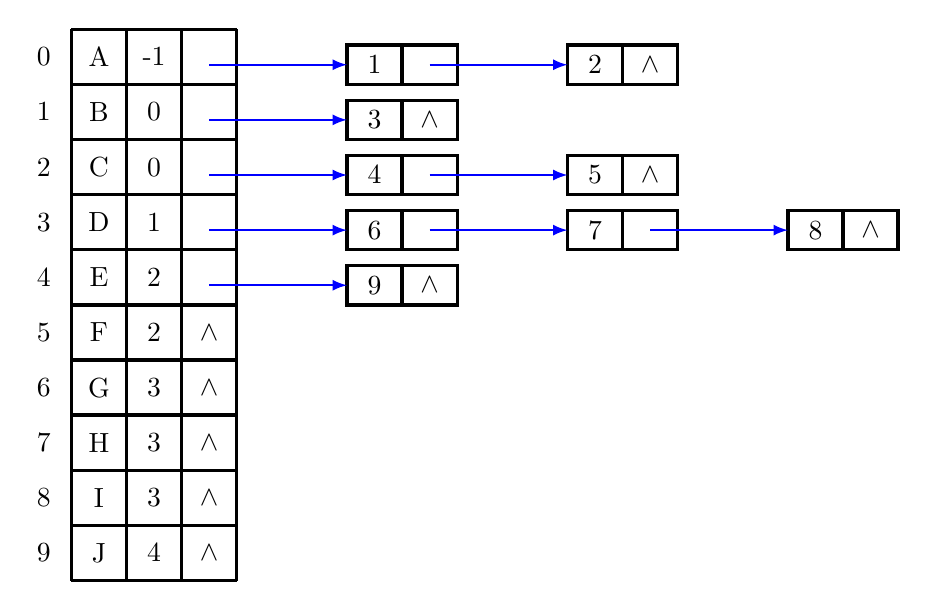
\begin{tikzpicture}[scale=1]
  \def\x{0.7} \def\y{0.7} \def\yy{0.5}
  %% \draw[dashed,step=\x] (0*\x,0*\y) grid (16*\x,10*\y);
  
  \draw[very thick,step=\x] (1*\x,0*\y) grid (4*\x,10*\y);
  \foreach \i in {0,1,2,...,9}
  \node at(0.5*\x,9.5*\y-\i*\y)[]{\i};

  \def\i{6}
  \foreach \j in {9,8,7,6,5}
  \draw[very thick,step=\x] (\i*\x,\j*\y) rectangle (\i*\x+2*\x,\j*\y+\yy)
  (\i*\x+\x,\j*\y)--(\i*\x+\x,\j*\y+\yy);

  \def\i{10}
  \foreach \j in {9,7,6}
  \draw[very thick,step=\x] (\i*\x,\j*\y) rectangle (\i*\x+2*\x,\j*\y+\yy)
  (\i*\x+\x,\j*\y)--(\i*\x+\x,\j*\y+\yy);

  \def\i{14}
  \foreach \j in {6}
  \draw[very thick,step=\x] (\i*\x,\j*\y) rectangle (\i*\x+2*\x,\j*\y+\yy)
  (\i*\x+\x,\j*\y)--(\i*\x+\x,\j*\y+\yy);
  
  \node at(1.5*\x,0.5*\y)[]{J}; \node at(2.5*\x,0.5*\y)[]{4}; 
  \node at(1.5*\x,1.5*\y)[]{I}; \node at(2.5*\x,1.5*\y)[]{3}; 
  \node at(1.5*\x,2.5*\y)[]{H}; \node at(2.5*\x,2.5*\y)[]{3}; 
  \node at(1.5*\x,3.5*\y)[]{G}; \node at(2.5*\x,3.5*\y)[]{3}; 
  \node at(1.5*\x,4.5*\y)[]{F}; \node at(2.5*\x,4.5*\y)[]{2}; 
  \node at(1.5*\x,5.5*\y)[]{E}; \node at(2.5*\x,5.5*\y)[]{2}; \node at(6.5*\x,5*\y+0.5*\yy)[]{9};  
  \node at(1.5*\x,6.5*\y)[]{D}; \node at(2.5*\x,6.5*\y)[]{1}; \node at(6.5*\x,6*\y+0.5*\yy)[]{6}; \node at(10.5*\x,6*\y+0.5*\yy)[]{7}; \node at(14.5*\x,6*\y+0.5*\yy)[]{8}; 
  \node at(1.5*\x,7.5*\y)[]{C}; \node at(2.5*\x,7.5*\y)[]{0}; \node at(6.5*\x,7*\y+0.5*\yy)[]{4}; \node at(10.5*\x,7*\y+0.5*\yy)[]{5}; 
  \node at(1.5*\x,8.5*\y)[]{B}; \node at(2.5*\x,8.5*\y)[]{0}; \node at(6.5*\x,8*\y+0.5*\yy)[]{3}; 
  \node at(1.5*\x,9.5*\y)[]{A}; \node at(2.5*\x,9.5*\y)[]{-1}; \node at(6.5*\x,9*\y+0.5*\yy)[]{1}; \node at(10.5*\x,9*\y+0.5*\yy)[]{2}; 

  \def\i{1}
  \foreach \j in {0,1,2,3,4}
  \node at(\i*\x+2.5*\x,\j*\y+0.5*\y)[]{$\land$};
  \foreach \j in {5,6,7,8,9}
  \draw[blue,thick,->,>=latex](\i*\x+2.5*\x,\j*\y+0.5*\yy)--(\i*\x+5*\x,\j*\y+0.5*\yy);

  \def\i{6}
  \foreach \j in {5,8}
  \node at(\i*\x+1.5*\x,\j*\y+0.5*\yy)[]{$\land$};
  \foreach \j in {6,7,9}
  \draw[blue,thick,->,>=latex](\i*\x+1.5*\x,\j*\y+0.5*\yy)--(\i*\x+4*\x,\j*\y+0.5*\yy);

  \def\i{10}
  \foreach \j in {9,7}
  \node at(\i*\x+1.5*\x,\j*\y+0.5*\yy)[]{$\land$};
  \foreach \j in {6}
  \draw[blue,thick,->,>=latex](\i*\x+1.5*\x,\j*\y+0.5*\yy)--(\i*\x+4*\x,\j*\y+0.5*\yy);

  \def\i{14}
  \foreach \j in {6}
  \node at(\i*\x+1.5*\x,\j*\y+0.5*\yy)[]{$\land$};

\end{tikzpicture}

\caption{孩子双亲表示法}
\end{figure}
\end{frame}
%
%
%
%\subsection{孩子兄弟表示法}
\begin{frame}\ft{孩子兄弟表示法}
\begin{wenti}
以上分别从双亲的角度和孩子的角度研究了树的存储结构,那么从树结点的兄弟的角度又会如何?
\end{wenti} \pause \vspace{0.1in}

对于树这样的层级结构来说,只研究结点的兄弟是不行的。\pause \vspace{0.1in}

\textcolor{acolor1}{任何一棵树,其结点的长子如果存在就是唯一的,它的大弟如果存在也是唯一的。因此,可设置两个指针,分别指向该结点的长子和右兄弟。}

\end{frame}
%
\begin{frame}\ft{孩子兄弟表示法}
\begin{figure}
\centering
\begin{tikzpicture}
  \def\x{2.5}\def\y{0.8}
  \draw[very thick](0,0)rectangle(3*\x,\y) (\x,0)--(\x,\y) (2*\x,0)--(2*\x,\y);
  \node at (0.5*\x,0.5*\y) [] {\tt data};
  \node at (1.5*\x,0.5*\y) [] {\tt firstchild};
  \node at (2.5*\x,0.5*\y) [] {\tt rightsib};

  \tikzstyle{every node}=[]
  \tikzstyle{information text}=[rounded corners,inner sep=1ex]
  \draw
  node at (1.5*\x,0*\y) [below=0.5cm,text width=10cm,style=information text]
  {
    \begin{table}
      \centering
      \begin{tabular}{l|l|l} \hline
         {\tt data} & 数据域 & 结点的数据信息 \\[0.1in]
         {\tt firstchild} & 指针域 &长子的存储地址\\[0.1in]
         {\tt rightsib} & 指针域 &大弟结点的存储地址 \\\hline
      \end{tabular}
      
    \end{table}
  };
\end{tikzpicture}

\caption{孩子兄弟表示法结构定义}
\end{figure}
\end{frame}
%
\begin{frame}\ft{孩子兄弟表示法}
\lstinputlisting[
language=C,
]{Chapters/Ch04/Code/Storage/sibling.h}
\end{frame}
%
%
\begin{frame}\ft{孩子兄弟表示法}
\begin{figure}
\centering
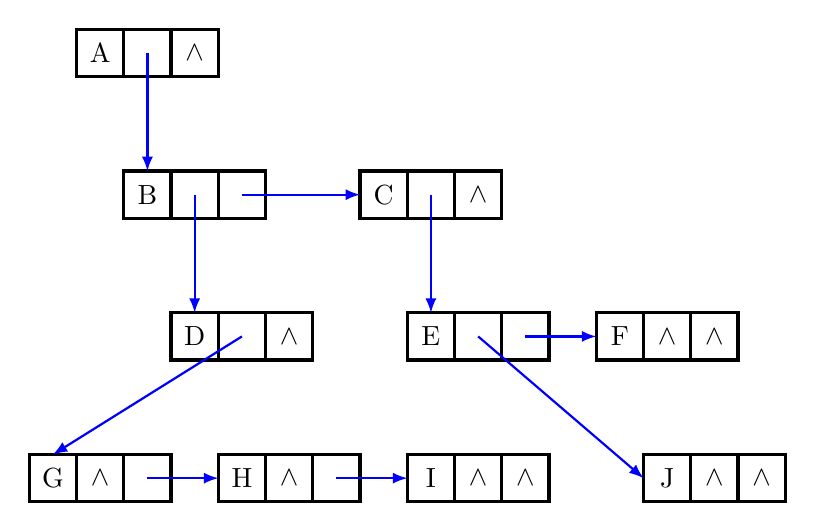
\begin{tikzpicture}[scale=1]
  \def\x{0.6} \def\y{0.6}
  %% \draw[dashed,step=\x] (0*\x,0*\y) grid (16*\x,12*\y);

  \foreach \i in {0,4,8,13}{
    \def\j{0}
    \draw[very thick](\i*\x,\j*\y)rectangle(\i*\x+3*\x,\j*\y+\y)
    (\i*\x+\x,\j*\y)--(\i*\x+\x,\j*\y+\y) (\i*\x+2*\x,\j*\y)--(\i*\x+2*\x,\j*\y+\y);
  }
  \def\i{0}\def\j{0}
  \node at(\i*\x+0.5*\x,\j*\y+0.5*\y)[]{G};
  \node at(\i*\x+1.5*\x,\j*\y+0.5*\y)[]{$\land$};

  \def\i{4}\def\j{0}
  \node at(\i*\x+0.5*\x,\j*\y+0.5*\y)[]{H};
  \node at(\i*\x+1.5*\x,\j*\y+0.5*\y)[]{$\land$};

  \def\i{8}\def\j{0}
  \node at(\i*\x+0.5*\x,\j*\y+0.5*\y)[]{I};
  \node at(\i*\x+1.5*\x,\j*\y+0.5*\y)[]{$\land$};
  \node at(\i*\x+2.5*\x,\j*\y+0.5*\y)[]{$\land$};

  \def\i{13}\def\j{0}
  \node at(\i*\x+0.5*\x,\j*\y+0.5*\y)[]{J};
  \node at(\i*\x+1.5*\x,\j*\y+0.5*\y)[]{$\land$};
  \node at(\i*\x+2.5*\x,\j*\y+0.5*\y)[]{$\land$};
  
  \foreach \i in {3,8,12}{
    \def\j{3}
    \draw[very thick](\i*\x,\j*\y)rectangle(\i*\x+3*\x,\j*\y+\y)
    (\i*\x+\x,\j*\y)--(\i*\x+\x,\j*\y+\y) (\i*\x+2*\x,\j*\y)--(\i*\x+2*\x,\j*\y+\y);
  }


  \def\i{3}\def\j{3}
  \node at(\i*\x+0.5*\x,\j*\y+0.5*\y)[]{D};
  \node at(\i*\x+2.5*\x,\j*\y+0.5*\y)[]{$\land$};

  \def\i{8}\def\j{3}
  \node at(\i*\x+0.5*\x,\j*\y+0.5*\y)[]{E};

  
  \def\i{12}\def\j{3}
  \node at(\i*\x+0.5*\x,\j*\y+0.5*\y)[]{F};
  \node at(\i*\x+1.5*\x,\j*\y+0.5*\y)[]{$\land$};
  \node at(\i*\x+2.5*\x,\j*\y+0.5*\y)[]{$\land$};

  \foreach \i in {2,7}{
    \def\j{6}
    \draw[very thick](\i*\x,\j*\y)rectangle(\i*\x+3*\x,\j*\y+\y)
    (\i*\x+\x,\j*\y)--(\i*\x+\x,\j*\y+\y) (\i*\x+2*\x,\j*\y)--(\i*\x+2*\x,\j*\y+\y);
  }

  \def\i{2}\def\j{6}
  \node at(\i*\x+0.5*\x,\j*\y+0.5*\y)[]{B};

  \def\i{7}\def\j{6}
  \node at(\i*\x+0.5*\x,\j*\y+0.5*\y)[]{C};
  \node at(\i*\x+2.5*\x,\j*\y+0.5*\y)[]{$\land$};


  \foreach \i in {1}{
    \def\j{9}
    \draw[very thick](\i*\x,\j*\y)rectangle(\i*\x+3*\x,\j*\y+\y)
    (\i*\x+\x,\j*\y)--(\i*\x+\x,\j*\y+\y) (\i*\x+2*\x,\j*\y)--(\i*\x+2*\x,\j*\y+\y);
  }
  \def\i{1}\def\j{9}
  \node at(\i*\x+0.5*\x,\j*\y+0.5*\y)[]{A};
  \node at(\i*\x+2.5*\x,\j*\y+0.5*\y)[]{$\land$};

  \draw[blue,thick,->,>=latex](2.5*\x,9.5*\y)--(2.5*\x,7.0*\y);
  \draw[blue,thick,->,>=latex](3.5*\x,6.5*\y)--(3.5*\x,4.0*\y);
  \draw[blue,thick,->,>=latex](8.5*\x,6.5*\y)--(8.5*\x,4.0*\y);
  \draw[blue,thick,->,>=latex](4.5*\x,6.5*\y)--(7.0*\x,6.5*\y);
  \draw[blue,thick,->,>=latex](4.5*\x,3.5*\y)--(0.5*\x,1.0*\y);
  \draw[blue,thick,->,>=latex](9.5*\x,3.5*\y)--(13*\x,0.5*\y);
  \draw[blue,thick,->,>=latex](10.5*\x,3.5*\y)--(12*\x,3.5*\y);
  \draw[blue,thick,->,>=latex](2.5*\x,0.5*\y)--(4.0*\x,0.5*\y);
  \draw[blue,thick,->,>=latex](6.5*\x,0.5*\y)--(8.0*\x,0.5*\y);
  
  
\end{tikzpicture}

%\caption{孩子兄弟表示法}
\end{figure}
\end{frame}
%
\begin{frame}\ft{孩子兄弟表示法}
该表示法便于查找某个结点的某个孩子。对于某个结点,可通过firstchild找到其长子,再通过长子的rightsib找到其二弟,接着一直找下去,直到找到具体的孩子。 \pause \vspace{0.1in}

若想找某个结点的双亲,该表示法也有缺陷。\vspace{0.05in}

可考虑再增加一个parent指针域来解决快速查找双亲的问题。

\end{frame}

\begin{frame}\ft{孩子兄弟表示法}
孩子兄弟表示法的最大好处是它把一颗复杂的树变成了一棵二叉树。
\end{frame}

\begin{frame}\ft{孩子兄弟表示法}
\begin{figure}
\centering
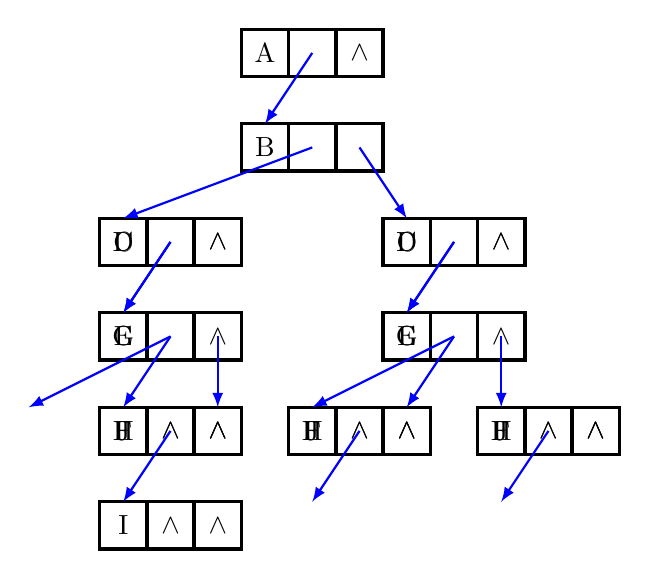
\begin{tikzpicture}[scale=1]
  \def\x{0.6} \def\y{0.6}
  %% \draw[dashed,step=\x] (0*\x,0*\y) grid (16*\x,11*\y);

  \foreach \i in {0}{
    \def\j{0}
    \draw[very thick](\i*\x,\j*\y)rectangle(\i*\x+3*\x,\j*\y+\y)
    (\i*\x+\x,\j*\y)--(\i*\x+\x,\j*\y+\y) (\i*\x+2*\x,\j*\y)--(\i*\x+2*\x,\j*\y+\y);
    \node at(\i*\x+0.5*\x,\j*\y+0.5*\y)[]{I};
    \node at(\i*\x+1.5*\x,\j*\y+0.5*\y)[]{$\land$};
    \node at(\i*\x+2.5*\x,\j*\y+0.5*\y)[]{$\land$};
  }

  \foreach \i in {0,4,8}{
    \def\j{2}
    \draw[very thick](\i*\x,\j*\y)rectangle(\i*\x+3*\x,\j*\y+\y)
    (\i*\x+\x,\j*\y)--(\i*\x+\x,\j*\y+\y) (\i*\x+2*\x,\j*\y)--(\i*\x+2*\x,\j*\y+\y);
    \ifthenelse{\i = 0} {
      \node at(\i*\x+0.5*\x,\j*\y+0.5*\y)[]{H};
      \draw[blue,thick,->,>=latex] (\i*\x+1.5*\x,\j*\y+0.5*\y)--(\i*\x+0.5*\x,\j*\y-\y);
      \node at(\i*\x+2.5*\x,\j*\y+0.5*\y)[]{$\land$};
    }{
      \ifthenelse{\i = 4} {
        \node at(\i*\x+0.5*\x,\j*\y+0.5*\y)[]{J};
        \node at(\i*\x+1.5*\x,\j*\y+0.5*\y)[]{$\land$};
        \node at(\i*\x+2.5*\x,\j*\y+0.5*\y)[]{$\land$};
      }{
        \node at(\i*\x+0.5*\x,\j*\y+0.5*\y)[]{F};
        \node at(\i*\x+1.5*\x,\j*\y+0.5*\y)[]{$\land$};
        \node at(\i*\x+2.5*\x,\j*\y+0.5*\y)[]{$\land$};
      }
    }
  }
  \foreach \i in {0,6}{
    \def\j{4}
    \draw[very thick](\i*\x,\j*\y)rectangle(\i*\x+3*\x,\j*\y+\y)
    (\i*\x+\x,\j*\y)--(\i*\x+\x,\j*\y+\y) (\i*\x+2*\x,\j*\y)--(\i*\x+2*\x,\j*\y+\y);
    \ifthenelse{\i = 0} {
      \node at(\i*\x+0.5*\x,\j*\y+0.5*\y)[]{G};
      \draw[blue,thick,->,>=latex] (\i*\x+1.5*\x,\j*\y+0.5*\y)--(\i*\x+0.5*\x,\j*\y-\y);
      \node at(\i*\x+2.5*\x,\j*\y+0.5*\y)[]{$\land$};
    }{
      \node at(\i*\x+0.5*\x,\j*\y+0.5*\y)[]{E};
      \draw[blue,thick,->,>=latex] (\i*\x+1.5*\x,\j*\y+0.5*\y)--(\i*\x-1.5*\x,\j*\y-\y);
      \draw[blue,thick,->,>=latex] (\i*\x+2.5*\x,\j*\y+0.5*\y)--(\i*\x+2.5*\x,\j*\y-\y);
    };
  }
  
  \foreach \i in {0,6}{
    \def\j{6}
    \draw[very thick](\i*\x,\j*\y)rectangle(\i*\x+3*\x,\j*\y+\y)
    (\i*\x+\x,\j*\y)--(\i*\x+\x,\j*\y+\y) (\i*\x+2*\x,\j*\y)--(\i*\x+2*\x,\j*\y+\y);
    \ifthenelse{\i = 0} {
      \node at(\i*\x+0.5*\x,\j*\y+0.5*\y)[]{D};
      \draw[blue,thick,->,>=latex] (\i*\x+1.5*\x,\j*\y+0.5*\y)--(\i*\x+0.5*\x,\j*\y-\y);
      \node at(\i*\x+2.5*\x,\j*\y+0.5*\y)[]{$\land$};
    }{
      \node at(\i*\x+0.5*\x,\j*\y+0.5*\y)[]{C};
      \draw[blue,thick,->,>=latex] (\i*\x+1.5*\x,\j*\y+0.5*\y)--(\i*\x+0.5*\x,\j*\y-\y);
      \node at(\i*\x+2.5*\x,\j*\y+0.5*\y)[]{$\land$};
    };
  }


  \foreach \i in {3}{
    \def\j{8}
    \draw[very thick](\i*\x,\j*\y)rectangle(\i*\x+3*\x,\j*\y+\y)
    (\i*\x+\x,\j*\y)--(\i*\x+\x,\j*\y+\y) (\i*\x+2*\x,\j*\y)--(\i*\x+2*\x,\j*\y+\y);
    \node at(\i*\x+0.5*\x,\j*\y+0.5*\y)[]{B};
    \draw[blue,thick,->,>=latex] (\i*\x+1.5*\x,\j*\y+0.5*\y)--(\i*\x-2.5*\x,\j*\y-\y);
    \draw[blue,thick,->,>=latex] (\i*\x+2.5*\x,\j*\y+0.5*\y)--(\i*\x+3.5*\x,\j*\y-\y);
  }

  \foreach \i in {3}{
    \def\j{10}
    \draw[very thick](\i*\x,\j*\y)rectangle(\i*\x+3*\x,\j*\y+\y)
    (\i*\x+\x,\j*\y)--(\i*\x+\x,\j*\y+\y) (\i*\x+2*\x,\j*\y)--(\i*\x+2*\x,\j*\y+\y);
    \node at(\i*\x+0.5*\x,\j*\y+0.5*\y)[]{A};
    \draw[blue,thick,->,>=latex] (\i*\x+1.5*\x,\j*\y+0.5*\y)--(\i*\x+0.5*\x,\j*\y-\y);
    \node at(\i*\x+2.5*\x,\j*\y+0.5*\y)[]{$\land$};
  }

  
  
\end{tikzpicture}

% \caption{孩子兄弟表示法:二叉树}
\end{figure}
\end{frame}
